\section{GNSS in Mobile Devices}
%
Welcome to this \LaTeX\ template. Here, we will introduce you to some basic features available in \LaTeX\ through Overleaf that you will need to write your lab report. For more information, you can read Overleaf guides by clicking \href{https://www.overleaf.com/learn}{here}. 
%
\subsection{Content}
The report should include a brief description of the tasks you performed, along with the results obtained and a discussion of the results. Please do not include content from the theory classes, it is not necessary to explain the background of the labs. The most important content for the report is the \textbf{analysis and discussion of the results you obtained}.
%
\subsection{Writing}
%
Avoid using expressions such as "in the Figure \textsc{below/above}" or "in the \textsc{following} Figure/Table/Algorithm". Unless specified otherwise, LaTeX adjusts the position of objects depending on the page content, so a Figure may appear before its reference in the text even if you inserted it after. Instead, use explicit references to objects (e.g., "in Figure 4") using the proper LaTeX commands. \\
Here is a list of general language tips for writing scientific reports: 
\begin{itemize}
    \item Avoid the use of contractions (e.g., don’t, can’t) or slang terms.
    \item Use a consistent spelling of words (e.g., British English or American English).
    \item We discourage the use of terms such as "obviously", "clearly" and other subjective or ambiguous adverbs. 
    \item Similarly, we suggest avoiding adjectives such as "huge", "impressive" or "great"; try to express quantities directly instead. \\
\end{itemize}
%
\subsection{Figures}
Figures can be added using the \textbackslash includegraphics command inside the \textsc{figure} environment.
%
\begin{figure}[H]
    \centering
    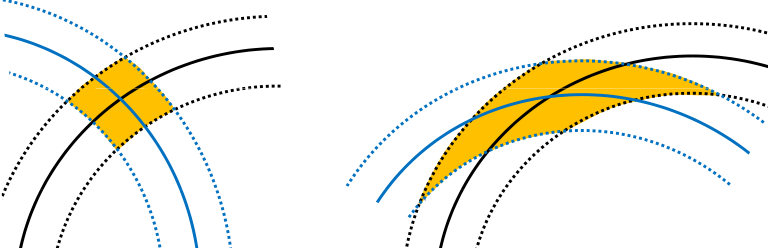
\includegraphics[width=0.6\textwidth]{Images/DOP_example.png}
    \caption{Example of \gls{DOP} in 2D positioning \cite{ESA:navi}.}
    \label{fig:DOP_example}
\end{figure}
%
Remember that in case you add plots, \textbf{axes should include proper labels and measurement units}. The figure should also include a caption with a brief description of its content. Furthermore, it is good practice to always reference a figure in the text using the command \textbackslash ref like this: Figure \ref{fig:DOP_example} using the proper label name. \\
We suggest to avoid including screenshots unless strictly necessary. Instead, you can include properly exported MATLAB figures (File $\rightarrow$ Save As). In order to get the best looking results, we suggest using vector graphics formats such as ".eps" (note: these formats may take longer for \LaTeX\ to compile). When instead using raster formats such as ".png" or ".jpg", be careful to export images with a sufficiently large resolution, so they will look nicely in your report. \\
%
\subsection{Citations}
If some material is taken from external sources, they should be cited using the command \textbackslash cite, as done for the caption of Figure \ref{fig:DOP_example}. The references need to be added first to the bibliography (.bib) file with the proper format, and then they can be cited from the text. Other useful resources and information for your report can be found in \cite{GOV:gps, ESA:navi}.
%
\subsection{Equations}
Here is how to write an equation in LaTeX:
%
\begin{equation}
    \frac{\partial u_i}{\partial t} + u_j \frac{\partial u_i}{\partial x_j} = -\frac{1}{\rho} \frac{\partial P}{\partial x_i} + \nu \frac{\partial^2 u_i}{\partial x_j^2}
    \label{eq:Navier-Stokes}
\end{equation}
%
A comprehensive guide of symbols, operators and other math commands can be found at \cite{LATEX:math}.
Differently from figures, you do not need to always reference equations in the text, but in case you need to, you can use the command \textbackslash eqref like this: \eqref{eq:Navier-Stokes}. \\
To add equations or numerical values with units inside the text you can use math mode within dollar signs \$, for example: speed of $\SI{10}{\meter \per \second}$. Math mode should also be used to insert mathematical symbols, for example: $\alpha$.
%
\subsection{Glossary}
Some commonly used acronyms have already been included in this template for your convenience. To define new acronyms, you can use the command \textbackslash newacronym in the "acronyms.tex" file. It is suggested to call acronyms in the text with the command \textbackslash gls like this: \gls{GNSS}, which will expand the acronym only on its first use. 
%
\subsection{Tables}
Tables can be inserted using the \textsc{table} and \textsc{tabular} environments.
%
\begin{table}[ht]
    \centering
    \begin{tabular}{c c c} 
        \toprule
        \textbf{State} & \textbf{LS} & \textbf{WLS} \\ 
        \midrule
        3D Position & 2.084 & 1.613 \\ 
        3D Velocity & 0.371 & 0.304 \\ 
        Clock Bias & 1.089 & 0.766 \\
        Clock Drift & 0.217 & 0.173 \\
        \bottomrule
    \end{tabular}
    \caption{Comparison of \gls{RMSE} between \gls{LS} and \gls{WLS}.}
    \label{tab:values}
\end{table} 
%
Once again, they should always be referenced in the text using the command \textbackslash ref like this: Table \ref{tab:values}.
%
\subsubsection{Results}
Please present your results in a quantitative (numerical) way using a suitable metric (e.g. \gls{RMSE} etc.). If required by the task, you may also present your results in a qualitative way (plots) but the numerical result should also be included. If a given task is to be repeated many times, it is suggested to not include too many plots and instead summarize the results in a table.
%